\documentclass{article}

\usepackage{graphics}

\begin{document}

\title{Scientific paper: standard article document class}
\author{John Smith \and Jan Kowalski}
\maketitle

\begin{abstract}
Lorem ipsum dolor sit amet, consectetur adipiscing elit. Donec id felis ipsum,
nec rutrum ipsum. Nam leo neque, venenatis in dignissim in, condimentum vel
nisl. Nam ornare tellus velit. Pellentesque varius rhoncus nisl et accumsan.
Aenean arcu risus, luctus sit amet aliquam nec, tincidunt at dui. Ut hendrerit
sem ut tellus condimentum congue. In hac habitasse platea dictumst. Vivamus
egestas, augue quis ultrices fermentum, leo nulla aliquet velit, eu congue est
tellus nec neque. Praesent tempus congue tellus, fringilla dapibus nisl
scelerisque nec.
\end{abstract}

\section{Introduction}
\label{sec:intro}
Mauris diam eros, tristique in vulputate eget, malesuada at metus. Nulla
facilisi. Vestibulum aliquet eleifend augue et porttitor. Nunc ac odio sit amet
dolor adipiscing rutrum at ac ligula. Morbi feugiat tempus felis sed molestie.
Maecenas ut molestie justo. Quisque eget diam in turpis porttitor congue. Donec
tempus, urna ac pretium aliquam, turpis enim eleifend turpis, eget vehicula
mauris nisl rhoncus mi. Nunc vitae libero sit amet justo scelerisque bibendum
in eget dui. Sed tincidunt, diam sed elementum ullamcorper, dui nunc
pellentesque purus, sed euismod lorem risus sit amet elit. Proin auctor metus
eget elit posuere ullamcorper \cite{smith.kowalski:running}.

\begin{figure}
  % GNUPLOT: LaTeX picture with Postscript
\begingroup
  \makeatletter
  \providecommand\color[2][]{%
    \GenericError{(gnuplot) \space\space\space\@spaces}{%
      Package color not loaded in conjunction with
      terminal option `colourtext'%
    }{See the gnuplot documentation for explanation.%
    }{Either use 'blacktext' in gnuplot or load the package
      color.sty in LaTeX.}%
    \renewcommand\color[2][]{}%
  }%
  \providecommand\includegraphics[2][]{%
    \GenericError{(gnuplot) \space\space\space\@spaces}{%
      Package graphicx or graphics not loaded%
    }{See the gnuplot documentation for explanation.%
    }{The gnuplot epslatex terminal needs graphicx.sty or graphics.sty.}%
    \renewcommand\includegraphics[2][]{}%
  }%
  \providecommand\rotatebox[2]{#2}%
  \@ifundefined{ifGPcolor}{%
    \newif\ifGPcolor
    \GPcolorfalse
  }{}%
  \@ifundefined{ifGPblacktext}{%
    \newif\ifGPblacktext
    \GPblacktexttrue
  }{}%
  % define a \g@addto@macro without @ in the name:
  \let\gplgaddtomacro\g@addto@macro
  % define empty templates for all commands taking text:
  \gdef\gplbacktext{}%
  \gdef\gplfronttext{}%
  \makeatother
  \ifGPblacktext
    % no textcolor at all
    \def\colorrgb#1{}%
    \def\colorgray#1{}%
  \else
    % gray or color?
    \ifGPcolor
      \def\colorrgb#1{\color[rgb]{#1}}%
      \def\colorgray#1{\color[gray]{#1}}%
      \expandafter\def\csname LTw\endcsname{\color{white}}%
      \expandafter\def\csname LTb\endcsname{\color{black}}%
      \expandafter\def\csname LTa\endcsname{\color{black}}%
      \expandafter\def\csname LT0\endcsname{\color[rgb]{1,0,0}}%
      \expandafter\def\csname LT1\endcsname{\color[rgb]{0,1,0}}%
      \expandafter\def\csname LT2\endcsname{\color[rgb]{0,0,1}}%
      \expandafter\def\csname LT3\endcsname{\color[rgb]{1,0,1}}%
      \expandafter\def\csname LT4\endcsname{\color[rgb]{0,1,1}}%
      \expandafter\def\csname LT5\endcsname{\color[rgb]{1,1,0}}%
      \expandafter\def\csname LT6\endcsname{\color[rgb]{0,0,0}}%
      \expandafter\def\csname LT7\endcsname{\color[rgb]{1,0.3,0}}%
      \expandafter\def\csname LT8\endcsname{\color[rgb]{0.5,0.5,0.5}}%
    \else
      % gray
      \def\colorrgb#1{\color{black}}%
      \def\colorgray#1{\color[gray]{#1}}%
      \expandafter\def\csname LTw\endcsname{\color{white}}%
      \expandafter\def\csname LTb\endcsname{\color{black}}%
      \expandafter\def\csname LTa\endcsname{\color{black}}%
      \expandafter\def\csname LT0\endcsname{\color{black}}%
      \expandafter\def\csname LT1\endcsname{\color{black}}%
      \expandafter\def\csname LT2\endcsname{\color{black}}%
      \expandafter\def\csname LT3\endcsname{\color{black}}%
      \expandafter\def\csname LT4\endcsname{\color{black}}%
      \expandafter\def\csname LT5\endcsname{\color{black}}%
      \expandafter\def\csname LT6\endcsname{\color{black}}%
      \expandafter\def\csname LT7\endcsname{\color{black}}%
      \expandafter\def\csname LT8\endcsname{\color{black}}%
    \fi
  \fi
  \setlength{\unitlength}{0.0500bp}%
  \begin{picture}(5668.00,3400.00)%
    \gplgaddtomacro\gplbacktext{%
      \csname LTb\endcsname%
      \put(726,440){\makebox(0,0)[r]{\strut{}-1}}%
      \put(726,710){\makebox(0,0)[r]{\strut{}-0.8}}%
      \put(726,979){\makebox(0,0)[r]{\strut{}-0.6}}%
      \put(726,1248){\makebox(0,0)[r]{\strut{}-0.4}}%
      \put(726,1518){\makebox(0,0)[r]{\strut{}-0.2}}%
      \put(726,1788){\makebox(0,0)[r]{\strut{} 0}}%
      \put(726,2057){\makebox(0,0)[r]{\strut{} 0.2}}%
      \put(726,2327){\makebox(0,0)[r]{\strut{} 0.4}}%
      \put(726,2596){\makebox(0,0)[r]{\strut{} 0.6}}%
      \put(726,2866){\makebox(0,0)[r]{\strut{} 0.8}}%
      \put(726,3135){\makebox(0,0)[r]{\strut{} 1}}%
      \put(858,220){\makebox(0,0){\strut{}-10}}%
      \put(1961,220){\makebox(0,0){\strut{}-5}}%
      \put(3065,220){\makebox(0,0){\strut{} 0}}%
      \put(4168,220){\makebox(0,0){\strut{} 5}}%
      \put(5271,220){\makebox(0,0){\strut{} 10}}%
    }%
    \gplgaddtomacro\gplfronttext{%
      \csname LTb\endcsname%
      \put(4284,2962){\makebox(0,0)[r]{\strut{}sin(x)}}%
    }%
    \gplbacktext
    \put(0,0){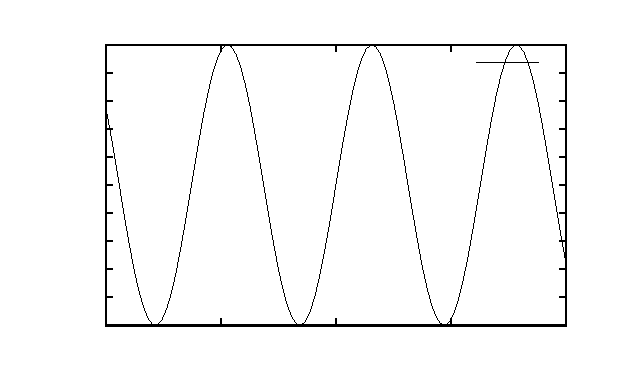
\includegraphics{sin}}%
    \gplfronttext
  \end{picture}%
\endgroup

  \caption{Example figure}
\end{figure}

Sed et orci lacus. Donec semper condimentum tempor. Aliquam id dolor quis nibh
consequat sollicitudin eu vel sapien. Phasellus eget est arcu, nec dignissim
lorem. Nunc pharetra leo at ligula dignissim quis viverra nibh varius. Proin
dui tortor, convallis vel dignissim nec, vestibulum id leo. Proin et lacus eu
lacus ultrices facilisis. Proin et elit libero, in volutpat leo. Etiam lorem
nulla, tempor et luctus auctor, tristique eget quam. Ut eget lorem vitae odio
tempus rutrum. Aliquam nec sem tortor. 

\section{Conclusions}
\label{sec:conclusions}

Lorem ipsum dolor sit amet, consectetur adipiscing elit. Sed at ligula lectus,
eget pretium lectus. Aenean ut libero libero. Nunc imperdiet mollis pretium.
Vestibulum in lorem vitae dolor dignissim hendrerit vitae at erat. Vivamus at
porttitor erat. Cras fringilla, dolor at facilisis tincidunt, leo eros volutpat
erat, ut facilisis neque diam quis quam. Duis vel nisi nunc. Suspendisse
laoreet tristique elit eu elementum. Sed pharetra porta velit consectetur
aliquet. Etiam nec nisl et purus tincidunt mattis. 

\bibliographystyle{plain}
\bibliography{$NAME}

\end{document}
% vim: set syntax=tex tabstop=2 shiftwidth=2 expandtab spell:
